
\documentclass[submit,techrep,noauthor]{ipsj}
%\documentclass{ipsj}

\usepackage[dvipdfmx]{graphicx}
\usepackage{latexsym}
\usepackage{cite}
\usepackage{subfigure}

\def\Underline{\setbox0\hbox\bgroup\let\\\endUnderline}
\def\endUnderline{\vphantom{y}\egroup\smash{\underline{\box0}}\\}
\def\|{\verb|}

\setcounter{巻数}{59} 
%\setcounter{号数}{1}
%\setcounter{page}{1}
\setcounter{year}{2020}


\受付{2020}{6}{26}
%\再受付{2015}{7}{16}   %省略可能
%\再再受付{2015}{7}{20} %省略可能
\採録{2020}{7}{30}


\newcommand{\fig}[1]{{図~\ref{fig:#1}}}
\newcommand{\tab}[1]{{表~\ref{tab:#1}}}
\newcommand{\ctext}[1]{\textcircled{\scriptsize{#1}}}

\graphicspath{{./figure/}}

\begin{document}


\title{容量効率を意識したソース・タグ値に基づく\\セグメント化による発行キューのエネルギー削減}

\affiliate{NU}{名古屋大学大学院工学研究科\\Graduate School of Engineering, Nagoya University}

\author{森 健一郎}{Kenichiro Mori}{NU}[mori@ando.nuee.nagoya-u.ac.jp]
\author{安藤 秀樹}{Hideki Ando}{NU}

\begin{abstract}
発行キューは電力密度の大きいホット・スポットとして知られている.ホット・スポットは,デバイスの摩耗故障を引き起こし,誤動作やタイミング・エラーを引き起こす.発行キューが大きな電力を消費する原因は,ウェイクアップ論理のタグ比較回路である.この回路はCAMで構成されており,全てのデスティネーション・タグと発行キュー内の全てのソース・タグとの多数の比較を一斉に行うため,非常に大きな電力を消費する.そこで本論文では,CAM の分野で提案されている手法を応用し,タグ比較による消費電力を削減する手法を提案する.本手法では,発行キューを複数のセグメントに分割する.命令は,ソース・タグの下位ビットがセグメント番号と一致するセグメントにディスパッチする.そして,ウェイクアップ時には,デスティネーション・タグの下位ビットが一致するセグメントにあるタグ比較器のみを動作させる.一致しないセグメントの比較器は動作しないため,タグ比較器の動作回数を削減できる.

本手法では,命令がディスパッチされるセグメントに空きがない場合,他のセグメントに空きがあってもディスパッチできないためストールする.この結果,発行キューの容量効率が低下するという問題が生じる.この問題は,発行キューの容量効率が重要なプログラムにおいて性能低下を引き起こす.そこで本論文では,容量効率を重視したディスパッチ・アルゴリズムと,タグ比較の積極的な削減を重視したディスパッチ・アルゴリズムを動的に切り替える手法を提案する.本手法は,発行キューの容量効率が重要な場合は容量効率の低下による性能低下を抑制し,そうでない場合は積極的にタグ比較器の動作回数を削減することを可能とする.提案手法を SPEC CPU 2017 を用いて評価を行った.結果,性能低下を最大で 5\% 以下(平均 -1\%)に抑えつつ,タグ比較器の動作回数を平均で 85\% 削減できることを確認した.
\end{abstract}

\maketitle

%1 はじめに
\section{はじめに}
現在のプロセッサは,非常に微細な LSI 技術で製造される.このような LSI の微細化に伴い,デバイスの信頼性低下の問題が深刻になっている~\cite{Weste2010}.微細化は,経年劣化や摩耗故障を加速し,その結果,タイミング・エラーや誤動作を引き起こし,デバイスの寿命を縮める.経年劣化や摩耗故障は温度に関して指数関数的に加速し~\cite{Monsieur2001,Khan2010,Black1969},温度10〜15℃の上昇でデバイスの寿命は半分以下になる~\cite{Viswanath2000}.

プロセッサ・チップ上には,ホット・スポットと呼ばれる単位面積あたりの電力が大きい場所が存在する.ホット・スポットは,そうでない場所と比べて温度上昇が激しいため,上述した故障を引き起こす確率が高くなる.従って,ホット・スポットを生成する回路の消費電力を低下させる必要がある.

ホット・スポットを生成する回路の1つに,発行キューがある.発行キューのサイズはプロセッサの世代が進むごとに大きくなっており,より深刻なホット・スポットとなっている.従って,発行キューの電力削減に対する要求は非常に大きい.
  
発行キューの中で最も電力を消費する回路は,タグ比較の回路である.タグ比較は,発行幅分のデスティネーション・タグとすべてのソース・タグとの間で行われるため,非常に多くの電力を消費する.そこで本論文では,タグ比較器が動作する回数を削減する以下のような手法を提案する.
\begin{itemize}
  \item 発行キューを複数の\textbf{セグメント}に分割する.命令を発行キューにディスパッチする際,第 1 ソース・タグの下位ビットが $n$ である命令は,第 $n$ 番目のセグメントに書き込む.タグ比較時には,デスティネーション・タグの下位ビットがセグメント番号と一致するセグメントでのみ,第 1 ソース・タグの比較を行う.一致しないセグメントでは比較が行われない.これによりタグ比較回数が削減される.
  \item 上記の方法では,第 2 ソース・タグの比較回数は削減されない.そこで提案手法では\textbf{スワップ}と\textbf{サブ・セグメント}と呼ぶ 2 つの方法を導入し,第 2 ソース・タグの比較回数も削減する.スワップは,ディスパッチ時に第 1 ソース・オペランドがレディで,第 2 ソース・オペランドがレディでない命令において,第 1 ソース・タグと第 2  ソース・タグを格納するフィールドを交換し,第 2 ソース・タグの下位ビットを用いてディスパッチするセグメントを決定する手法である.サブ・セグメントは,各セグメントを第 2 ソース・タグにもとづきさらに分割する手法である.
  \item セグメント化によりディスパッチできるエントリが制限されるため,発行キューの容量効率が低下し,容量に敏感なプログラムにおいて性能が低下するという問題が存在する.この問題に対応するため,本論文では \textbf{SWITCH} という手法を提案する.SWITCH では,容量効率を重視したディスパッチ・アルゴリズムと,タグ比較回数の削減を重視したディスパッチ・アルゴリズムを,容量効率の重要性に応じて切り替えて使用することにより,性能低下を抑制する.
\end{itemize}

提案手法を SPEC CPU 2017 ベンチマークを用いて評価し,性能低下を 最大でも 5\% 以下(平均 -1\%)に抑えつつ,タグ比較の回数を平均で 85\% 削減できることを確認した.

本論文の残りの構成は次の通りである.まず,\ref{sec:issue_queue}節で発行キューの基本的な事項を説明する.そして,\ref{sec:segmented_IQ}節で提案手法の基本となるアイデアに関して説明した後,\ref{sec:second_tag_comp}節で提案手法における第 2  ソース・タグのタグ比較回数削減方法に関して述べる.その後,\ref{sec:occupency_reduction}節で提案手法の問題点である発行キューの容量効率の低下に関して説明した後,\ref{sec:switch}節で容量効率の低下に対する対策方法を説明する.\ref{sec:eval}節で評価を行い,\ref{sec:summary}節でまとめる.

%2 発行キュー
\section{発行キュー}
\label{sec:issue_queue}
%%% 図中に IQ と表記しているので,abbreviation は残しています.
発行キュー(IQ : Issue Queue)はアウト・オブ・オーダ実行を行うプロセッサにおいて,リネームされた命令を保持し,実行順序をスケジューリングして,機能ユニットへ発行する回路である.本節では,発行キューの動作のうち,本研究において重要な,ディスパッチとウェイクアップに関して説明する.その後,発行キューの電力削減に関する関連研究を紹介する.

\subsection{発行キューの動作}
\subsubsection{ディスパッチ}
リネームされた命令は,発行キューにエントリが割り当てられ,命令の情報が格納される.この動作をディスパッチと呼ぶ.ディスパッチの動作は,発行キューの方式により異なる.過去には,プログラム順に命令を並べて格納するシフティング・キュー~\cite{Farrell1998}やサーキュラー・キュー~\cite{Abella:survey2003}が商用プロセッサで使われたが,近年では,回路の単純化や電力削減のため空いているエントリに単純にディスパッチするランダム・キューが使用されている.よって,命令の並びは年齢に関してランダムとなる.

ランダム・キューでは,発行キューの空きエントリのインデクスを保持するフリー・リストを用意する.ディスパッチ時には,フリー・リストから読み出したインデクスが指す発行キューのエントリに命令を書き込む.発行キューから命令が発行されエントリが無効化されると,そのインデクスをフリー・リストへ返す.フリー・リストは FIFO バッファで管理される.

\begin{figure}[tb]
  \centering
  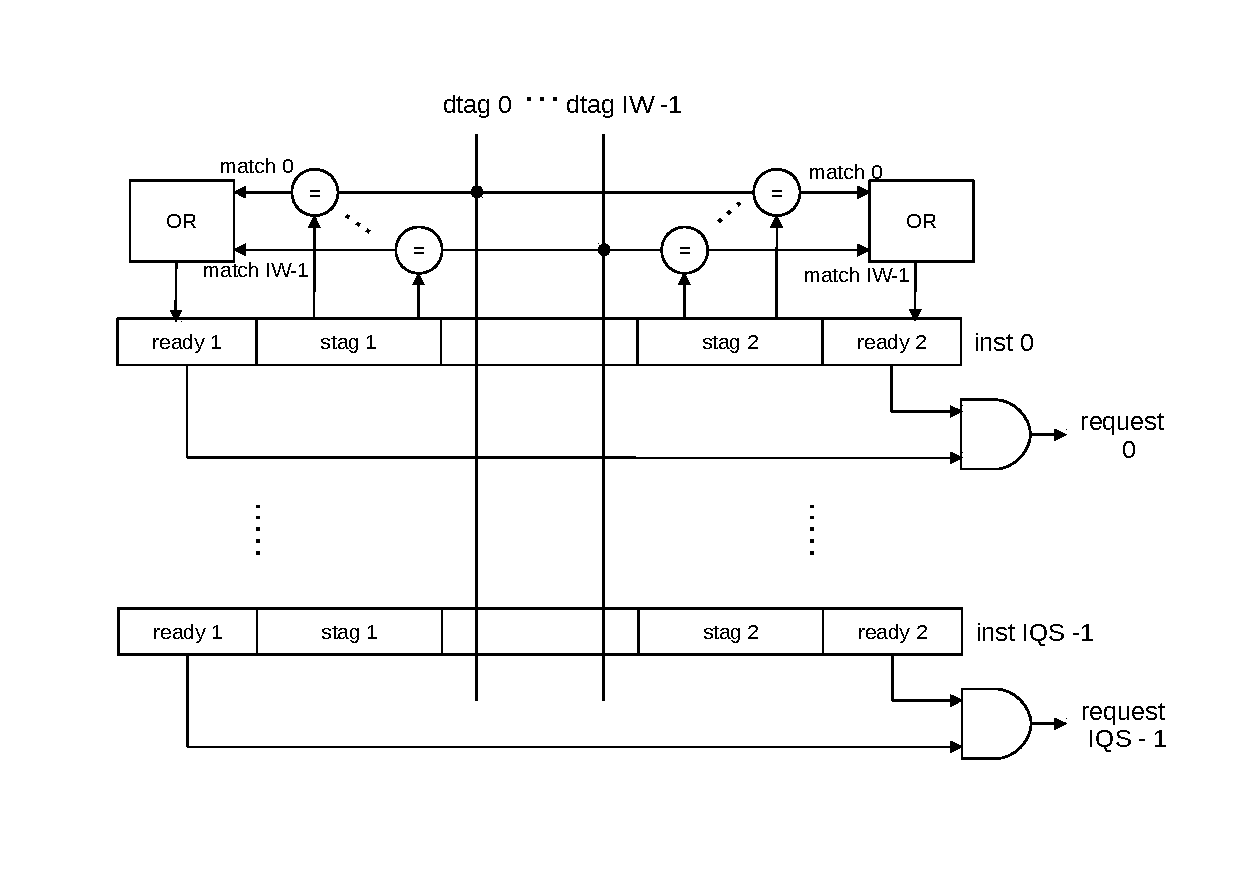
\includegraphics[keepaspectratio, scale=.8]{wakeup_logic.pdf}
  \caption{ウェイクアップ回路}
  \label{fig:wakeup_logic}
\end{figure}

\begin{figure}[tb]
  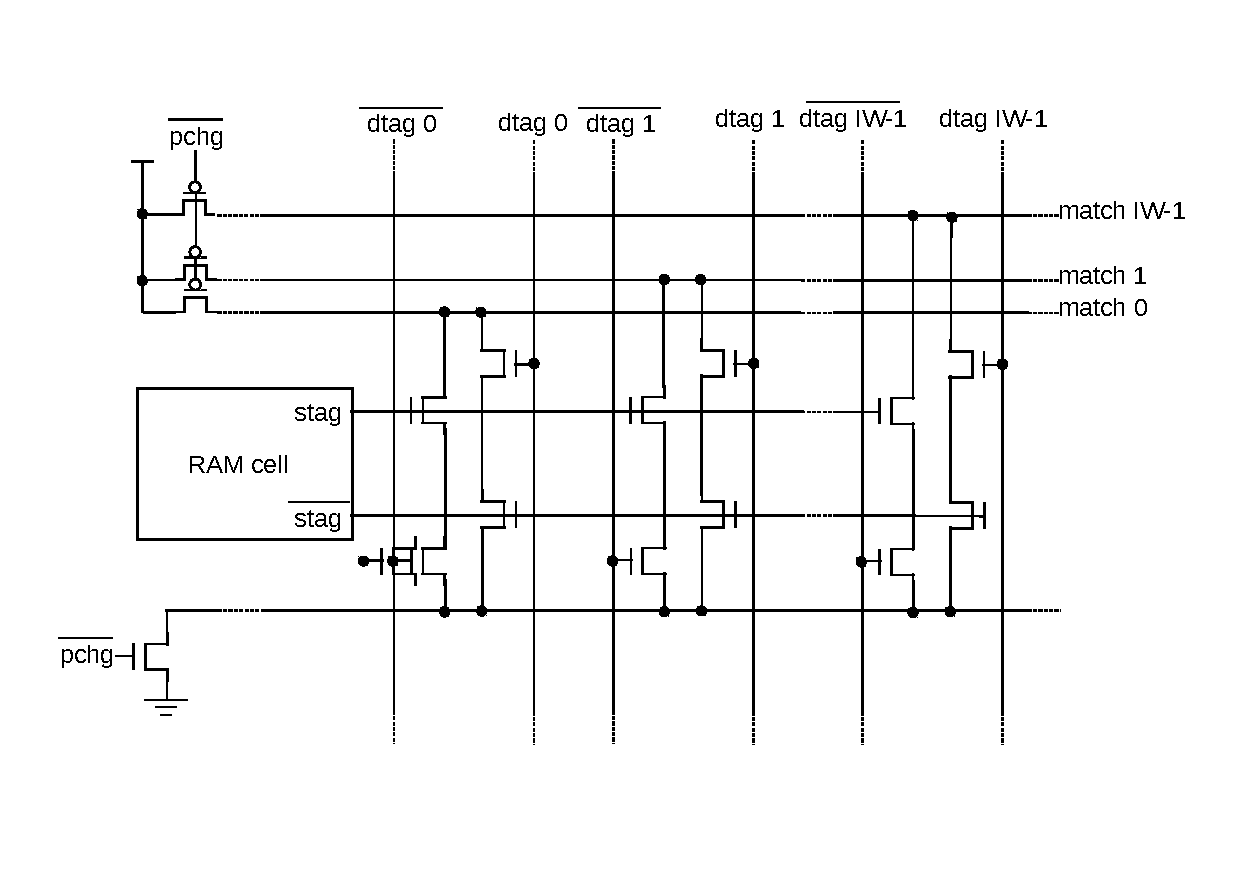
\includegraphics[keepaspectratio, scale=.8]{cam.pdf}
  \caption{タグ比較器の CAM 回路}
  \label{fig:cam}
\end{figure}

\subsubsection{ウェイクアップ}
命令が発行されると,その命令のデスティネーション・オペランドのタグと発行キュー内にある全命令のソース・オペランドのタグの比較が行われる.比較が一致した場合には,対応するソース・オペランドのレディ・ビットをセットする.この動作をウェイクアップと呼ぶ.両方のオペランドがレディとなった命令は,依存が解消したため発行可能となる.

\fig{wakeup_logic}に,ウェイクアップの回路を示す.図中の $IW$ は発行幅を,$IQS$ は発行キューのエントリ数を表す.ウェイクアップでは,$IW$ 個のデスティネーション・タグ(dtag)が発行キュー内の全命令に放送される.各命令は 2 つのソース・タグ(stag)を保持しており,放送されたデスティネーション・タグと比較が行われる.いずれかのデスティネーション・タグとソース・タグが一致した場合,そのソース・オペランドのレディ・ビットがセットされる.2 つのレディ・ビットがセットされた命令は発行が可能となるため発行要求が出力される.

\fig{cam}に発行キューに使用されるタグ比較器の CAM 回路を示す.同図は,ソース・タグ 1 ビット分の比較回路を表す.同図に示すように,高速化のため通常ダイナミック論理によって構成される.比較の動作は,次のように行われる.まず,マッチ線がプリチャージされる.次にデスティネーション・タグが放送され,比較が行われる.タグが不一致であれば,直列に接続された 2 つのプルダウン・トランジスタが両方とも ON となり,マッチ線がディスチャージされる.タグが一致する場合,マッチ線は $H$ の状態が維持される.比較器はマッチ線のディスチャージ時に電力を消費する.


\subsection{発行キューの電力削減に関する関連研究}
発行キューの電力削減に関する研究を紹介する.Ponomarev らは,リソース要求に応じて 発行キューのサイズをリサイズすることにより,消費エネルギーを削減する手法を提案した~\cite{ponomarev2001} .

Sembrant らは,クリティカル・パス上にない命令を発行キューとは別のバッファに入れ,ディスパッチを遅延させることによって,性能を低下させずに発行キューのサイズを小さくする手法を提案した~\cite{Sembrant2015}.

Ernst らは,発行キューを,2 つのソース・オペランドを保持できるキュー,1 つのソース・オペランドのみ保持できるキュー,オペランドを保持しないキューの 3 つに分割し,レディでないソース・オペランドの数に応じていずれかにディスパッチする手法を提案した~\cite{ernst2002}. この手法では,タグ比較器の数そのものを削減できるため,ウェイクアップの消費電力を削減できる.

Ponomarev らと Sembrant らの手法は,発行キューのサイズを縮小することによって電力削減を行うアプローチである.Ernst らの手法は,不要な比較器を削除することによって電力削減を行うアプローチである.これらの手法に対し本研究は,発行キューをタグの値によって配置分けし,これによりタグ比較の回数を削減し発行キューの電力削減を行うアプローチである.

%3 発行キューのセグメント化
\section{発行キューのセグメント化}
\label{sec:segmented_IQ}
本論文では,発行キューのタグ比較器の動作回数を削減するための手法として,発行キューをセグメント化する手法を提案する.本節では,まず提案手法の概要を説明した後,提案手法におけるウェイクアップとディスパッチに関して詳しく説明する.

\begin{figure}[htb]
  \centering
  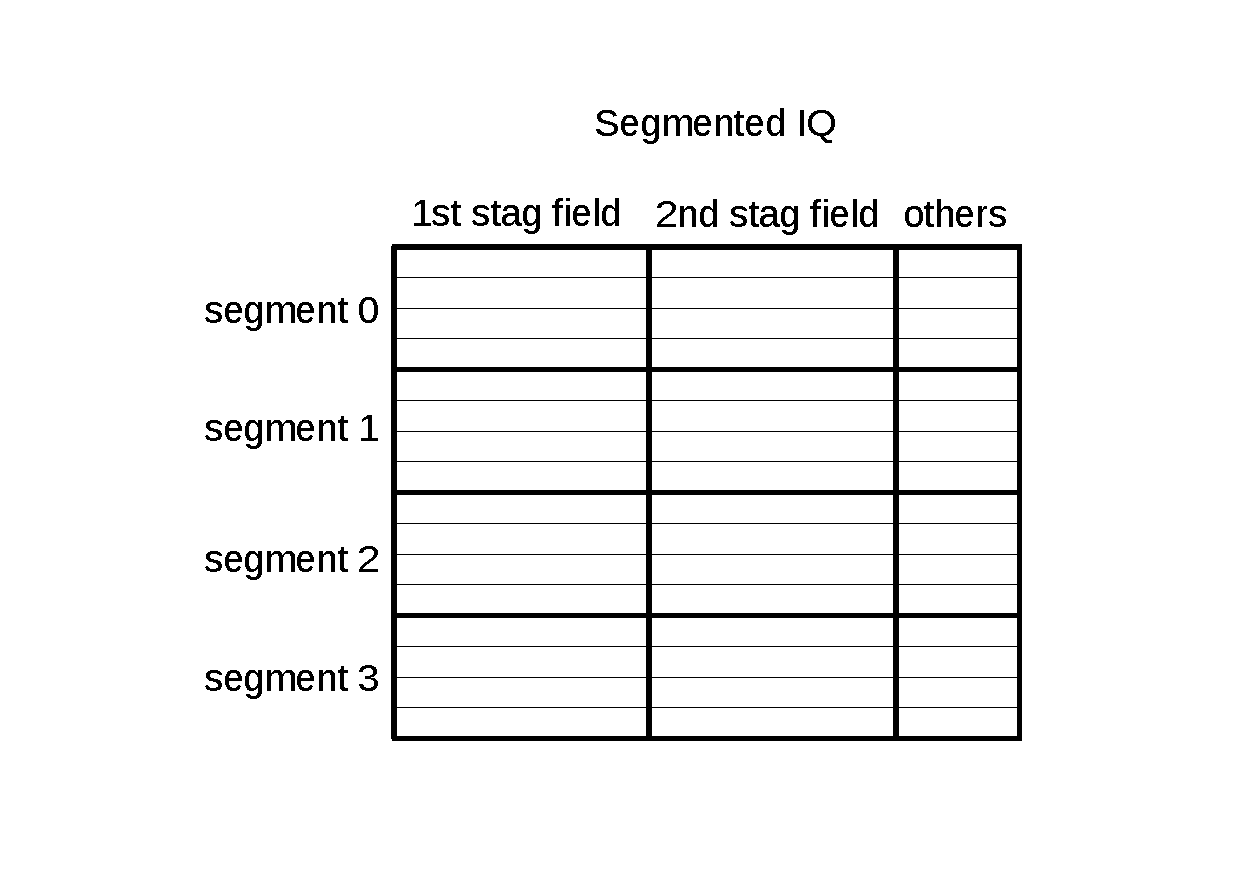
\includegraphics[keepaspectratio, scale=.8]{segmentedIQ.pdf}
  \caption{セグメント化した発行キュー}
  \label{fig:segmentedIQ}
\end{figure}

\subsection{提案手法の概要}
提案手法の基本アイデアは,大容量 CAM の電力削減に関する研究~\cite{Motomura1990journal}から着想を得ている.この研究において提案されている手法では,CAM を複数の\textbf{セグメント}~\footnote{文献~\cite{Motomura1990journal}ではバンクと呼ばれている}に分割する.各セグメントには下位ビットが同一のデータのみを記録する.そして,比較が行われる際には,比較対象のデータの下位ビットと,記録されているデータの下位ビットが一致するセグメントのみで比較を行う.これによって,比較器が動作する回数を「1/セグメント数」まで削減することができ,消費電力が削減できる.

本手法においても,\fig{segmentedIQ}に示すように発行キューを複数のセグメントに分割する.各セグメントには,第 1 ソース・タグの下位ビットがセグメントの番号と一致する命令をディスパッチする.ウェイクアップ時の第 1 ソース・タグのタグ比較では,デスティネーション・タグの下位ビットとセグメントの番号が一致するセグメントのみでタグ比較を行う.これによって,第 1 ソース・タグのタグ比較回数を「1/セグメント数」に削減できる.

提案手法におけるディスパッチとウェイクアップに関して詳しく説明する.

\begin{figure}[tb]
  \centering
  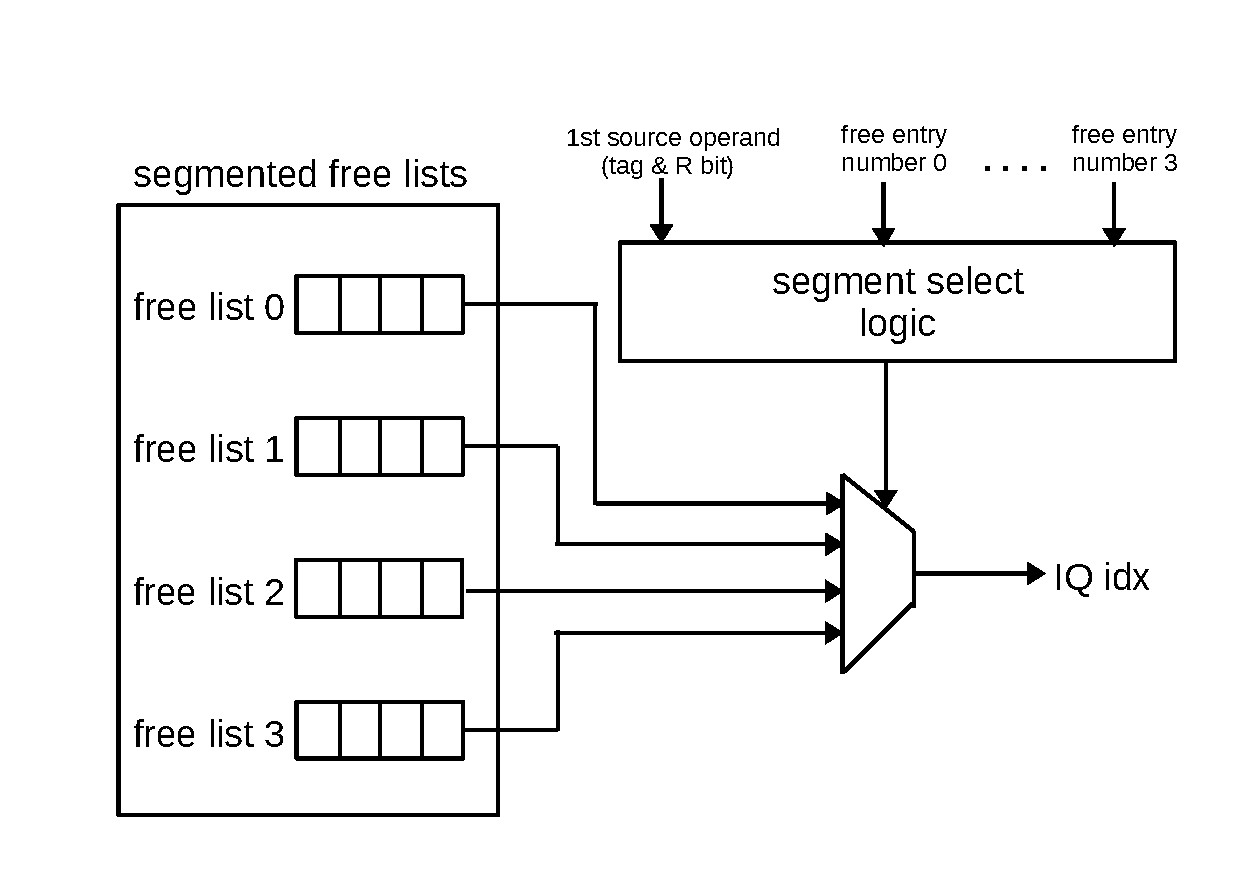
\includegraphics[keepaspectratio, scale=.8]{dispatch.pdf}
  \caption{提案手法におけるディスパッチエントリの決定回路}
  \label{fig:dispatch}
\end{figure}


\begin{figure*}[htb]
  \centering
  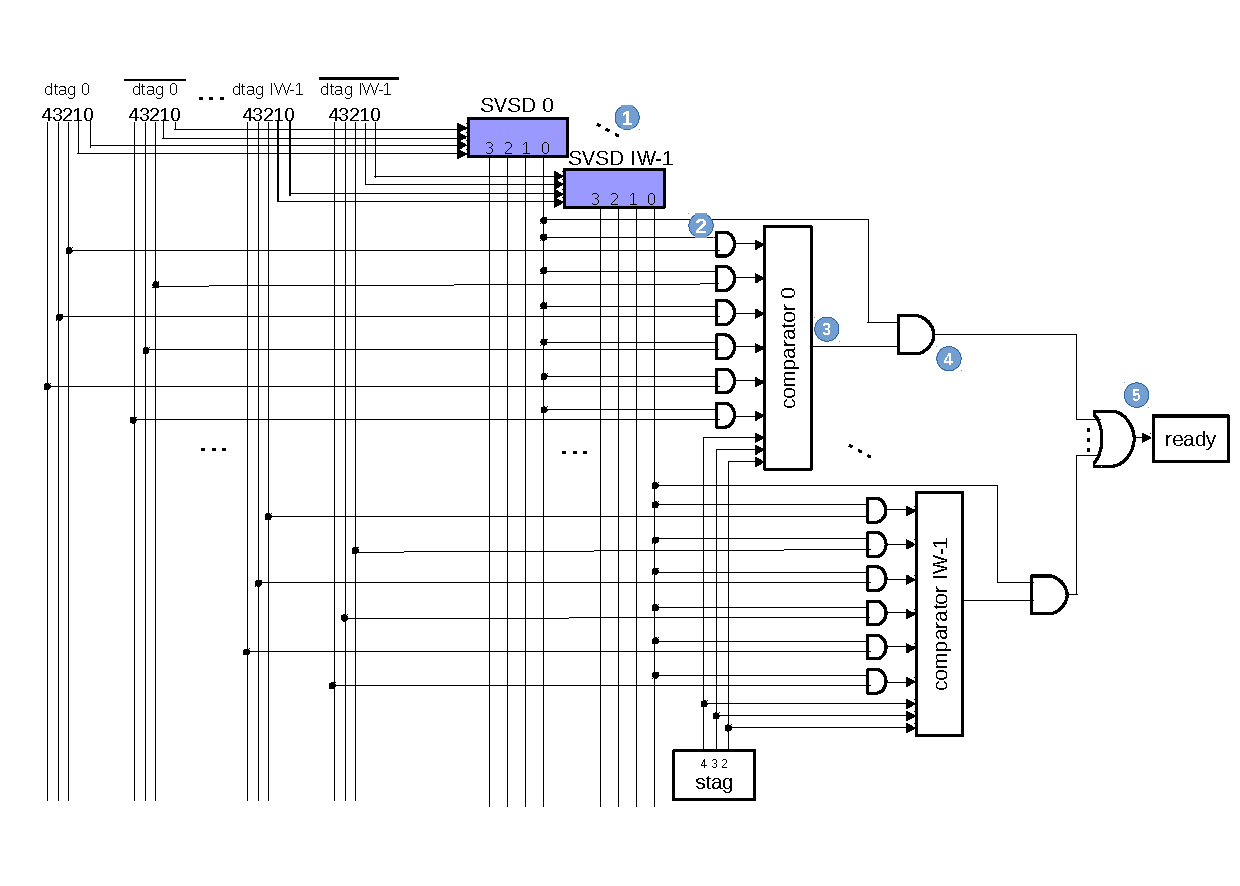
\includegraphics[width=0.80\hsize]{segmentedIQ_wakeup.pdf}
  \caption{提案手法におけるタグ比較回路(第 0 セグメント)}
  \label{fig:segmentedIQ_wakeup}
\end{figure*}

\subsection{提案手法におけるディスパッチ}
ディスパッチする発行キューのエントリを決定する回路を\fig{dispatch}に示す.本手法では,フリー・リストをセグメントと同じ数だけ用意する.各フリー・リストは,対応するセグメントの空きエントリのインデクスを FIFO バッファで管理する.各フリー・リストからは発行キューのインデクスが出力され,その中の1つを選択してディスパッチするエントリを決定する.どのフリー・リストからの出力を選択するかは,セグメント選択回路(図中の segment select logic)によって決定される.

セグメント選択回路の選択アルゴリズムについて説明する.セグメントの選択方法は,ディスパッチ時に第 1 ソース・オペランドがレディであるかによって異なるため,それぞれの場合に関して説明する.
\begin{itemize}
  \item \textbf{第 1 ソース・オペランドがレディでない場合}: 第 1 ソース・タグの下位ビットと番号が同じセグメントを選択する.選択されたセグメントに空きエントリがある場合,ディスパッチ可能であるため,対応するフリー・リストから読み出したエントリにディスパッチを行う.対応するセグメントに空きがない場合は,セグメントに空きが出るまでディスパッチをストールさせる.
  \item \textbf{第 1 ソース・オペランドがレディである場合}:この場合,第 1 ソース・タグの比較は行われないため,どのセグメントにディスパッチしても問題ない.このような場合を\textbf{セグメント・インディペンデント}と呼ぶ.セグメント・インディペンデントの場合,空きエントリのあるセグメントから,ラウンドロビンでディスパッチするセグメントを選択しディスパッチする.
\end{itemize}
例として,第 1 ソース・オペランドがレディでなく,タグが 15(${\rm 1111_2}$)である命令を,\fig{segmentedIQ}に示す 4 つに分割された発行キューにディスパッチする場合を考える.第 1 ソース・タグの下位 2 ビットが 3(${\rm 11_2}$)であるので,この命令は第 3 セグメントにディスパッチされる. 

なお,ソース・オペランドを使用しない命令も存在するが,そのような命令はディスパッチ時にソース・オペランドがレディであるものとして扱う.


\subsection{提案手法におけるウェイクアップ}
提案手法におけるウェイクアップでは,デスティネーション・タグの下位ビットがセグメント番号と一致するセグメントでのみ,第 1 ソース・タグのタグ比較器を動作させ比較を行う.一致しないセグメントはタグ比較器を動作させない.これは,デスティネーション・タグの下位ビットと番号が一致しないセグメントには,第 1 ソース・タグの下位ビットがデスティネーション・タグの下位ビットと異なる命令しか入っておらず,タグは必ず不一致となるためである.

例として,放送されたデスティネーション・タグが 6(${\rm 110_2}$)で,発行キューが\fig{segmentedIQ}のように 4 つのセグメントに分割されている場合を考える.この場合,下位ビットは 2(${\rm 10_2}$)であるため,第 2 セグメントでのみ,第 1 ソース・タグのタグ比較を行う.

なお,第 2 ソース・タグのタグ比較に関しては,セグメントの番号とタグの下位ビットに関係性はないため,すべてのセグメントでタグ比較を行う必要がある.

提案手法におけるタグ比較の回路を\fig{segmentedIQ_wakeup}に示す.同図は 4 つのセグメントに分割された発行キューのうち,第 0 セグメントのエントリにおける,第 1 ソース・タグの比較回路を示している.タグ・ビット数は 5 とし,発行幅を $IW$ とする.

タグ比較の動作を図中の番号を用いて説明する.\ctext{1}放送されるデスティネーション・タグの下位 2 ビットはデコーダへ送られる.デコーダはセグメント数だけ信号線を出力する.第 $n$ 番目の信号線は,第 $n$ セグメントでのタグ比較が有効であることを示す.つまり,デスティネーション・タグの下位ビットが $n$ の場合,$n$ 番目の出力線のみ $H$ を出力し,残りはすべて $L$ を出力する.

\ctext{2}AND ゲートによって,デコーダからの信号線が $H$ の場合にのみ,デスティネーション・タグの高位ビット及びその反転信号がタグ比較器へ入力される.\fig{segmentedIQ_wakeup}に示す回路は第 0 セグメントのタグ比較回路であるため,デコーダの 0 番目の信号線が AND ゲートに入力されている.

デコーダからの信号線が $H$ の場合,つまり,デスティネーション・タグの下位ビットとセグメント番号が一致していた場合のみ,比較器に有効なデスティネーション・タグの高位ビットとその反転信号が送られ,ソース・タグの高位ビットと比較が行われる.デコーダからの信号線が $L$ の場合,デスティネーション・タグとその反転信号がどちらも L としてタグ比較器へ入力される.この場合,デスティネーション・タグとその反転信号に接続されたプルダウン・トランジスタがすべて OFF となるため,マッチ線はディスチャージされず,電力を消費しない.

\ctext{3}タグ比較の結果,タグの高位ビットが一致した場合は,比較器から $H$ が出力される.

\ctext{4}タグ比較器が $H$ を出力し,かつデコーダからの信号が $H$ である場合に,タグ比較は一致となる.

\ctext{5}いずれかのデスティネーション・タグがソース・タグと一致した場合に,ソース・オペランドのレディ・ビットがセットされる.


%4 第 2 ソース・タグ比較の削減
\section{第 2 ソース・タグ比較の削減}
\label{sec:second_tag_comp}
\ref{sec:segmented_IQ}節で述べた手法では,命令の第 2 ソース・タグのタグ比較回数は削減できない.そこで本節では,第 2 ソース・タグの比較回数の削減を可能とする\textbf{スワップ}と\textbf{サブ・セグメント}という 2 つの手法を提案する.

\subsection{スワップ}
\label{sec:swap}
スワップは,第 1 ソース・タグと第 2 ソース・タグを格納するフィールドを交換し,第 2 ソース・タグの下位ビットをもとにディスパッチするセグメントを決定する手法である.以下で詳しく説明する.

第 1 ソース・オペランドがレディで,第 2 ソース・オペランドがレディでない場合について説明する.この場合,\ref{sec:segmented_IQ}節で説明した方法では,命令はセグメント・インディペンデントとしてディスパッチされる.第 1 ソース・オペランドは既にレディであるため,比較は第 2 ソース・タグについてのみ行われるが,第 2  ソース・タグのタグ比較は全てのセグメントで行われるため,タグ比較の回数は削減されない.

そこでこのような場合に,第 1 ソース・タグと第 2 ソース・タグを交換し(スワップ),第 2 ソース・タグの下位ビットを使用してディスパッチするセグメントを選択する.これにより,\ref{sec:segmented_IQ}節で述べたセグメント化の効果でタグ比較回数が削減される.なお,スワップではタグを交換するが,ペイロード RAM に格納するソース・タグを交換するわけではないので,命令の意味は保持される.

\subsubsection{スワップを行う場合のセグメント選択アルゴリズム}
セグメント選択回路は,以下に示すアルゴリズムによってディスパッチするセグメントを決定する.
\begin{itemize}
  \item \textbf{両ソース・オペランドともレディでない場合}:第 1 ソース・タグでセグメントを選択する.
  \item \textbf{第 1 ソース・オペランドのみレディである場合}:スワップを行い,第 2 ソース・タグでセグメントを選択する.
  \item \textbf{第 2 ソース・オペランドのみレディである場合}:第 1 ソース・タグでセグメントを選択する.
  \item \textbf{両ソース・オペランドがレディである場合}:セグメント・インディペンデントとしてラウンドロビンでセグメントを選択する.
\end{itemize}
なお,両ソース・オペランドがレディのとき以外で,選択されたセグメントに空きがない場合は,ディスパッチをストールして当該のセグメントに空きが出るまで待ち合わせる.

\begin{figure}[htb]
  \centering
  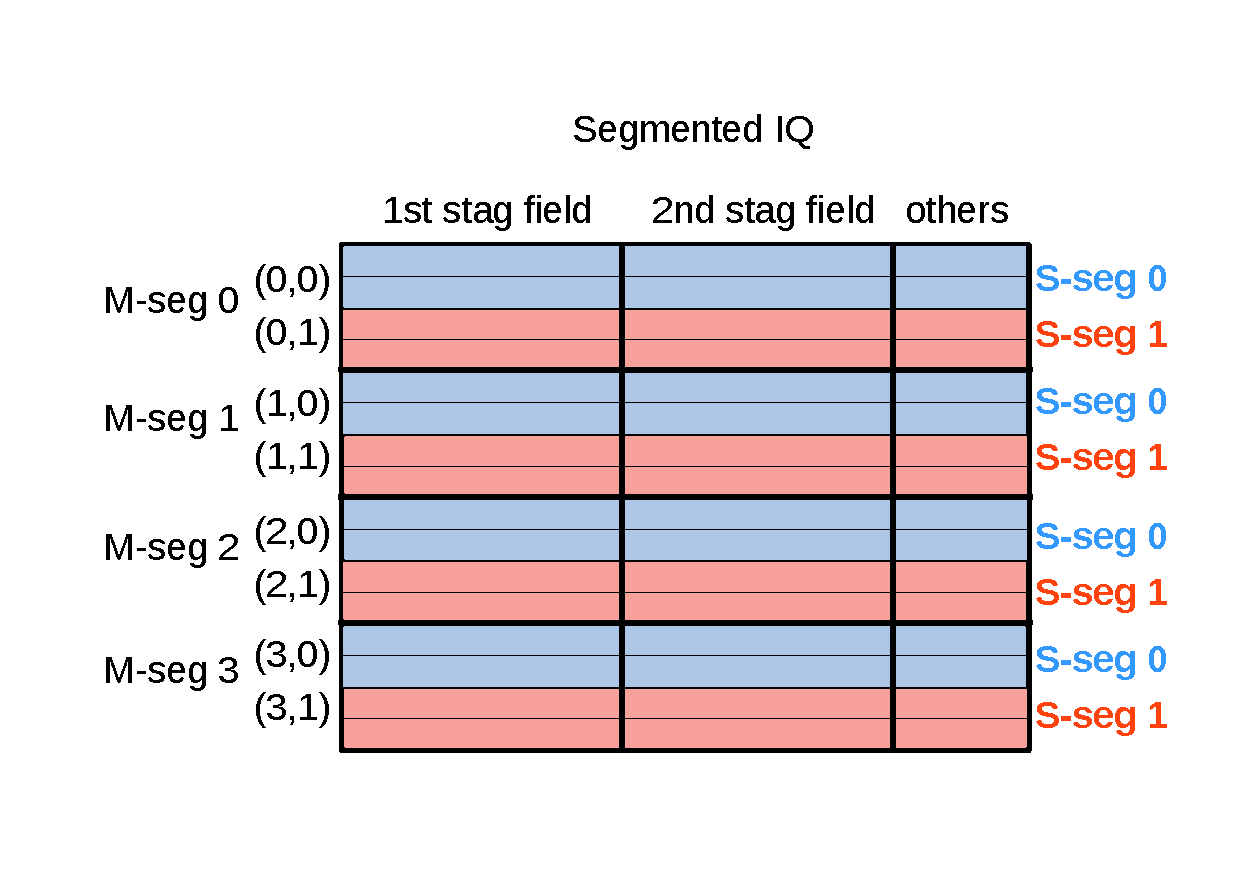
\includegraphics[keepaspectratio, scale=.8]{sub_segment.pdf}
  \caption{サブ・セグメントを実装した発行キュー}
  \label{fig:sub_segment}
\end{figure}

\subsection{サブ・セグメント}
\label{sec:sub_segment}
サブ・セグメント方式は,第 1 ソース・タグの下位ビットに応じて分割されるセグメントを,第 2 ソース・タグの下位ビットに応じてさらに細かく分割する.第 2 ソース・タグの下位ビットによる分割をサブ・セグメント(S-seg)と呼び,従来の第 1 ソース・タグによる分割をサブ・セグメントに対応してメイン・セグメント(M-seg)と呼ぶこととする.

サブ・セグメントを導入した発行キューの分割を\fig{sub_segment}に示す.黒色の枠で示す各メイン・セグメントを,赤色と青色で示すようにさらにサブ・セグメントに分割する.同図は,メイン・セグメント数が 4 ,サブ・セグメント数が 2 の場合の例を表している.各セグメントの左には,(M-seg, S-seg)という形式でメイン及びサブ・セグメントの番号を表している.

サブ・セグメント方式について,ディスパッチとウェイクアップの動作をそれぞれ説明する.

\subsubsection{サブ・セグメントにおけるディスパッチ}
サブ・セグメント方式におけるディスパッチにおいては,フリー・リストを M-seg $\times$ S-seg だけ用意する.\fig{sub_segment}に示した例の場合 8 個のフリー・リストが必要となる.

サブ・セグメント方式におけるセグメント選択のアルゴリズムに関して説明する.アルゴリズムはソース・オペランドのレディ状況によって異なるため,以下ですべての場合に関して説明する.説明を簡単にするため,命令 $p5 = p13 + p6$ を,\fig{sub_segment}に示す発行キューにディスパッチする場合について例示する.第 1 ソース・タグが 13 で,第 2 ソース・タグが 6 である.
\begin{itemize}
  \item \textbf{両ソース・オペランドともレディでない場合}:第 1 ソース・タグでメイン・セグメントを,第 2 ソース・タグでサブ・セグメントを選択する.例の場合,第 1 ソース・タグ 13(${\rm 1101_2}$) の下位ビット 1(${\rm 01_2}$)より,メイン・セグメントは 1 となる.また,第 2 ソース・タグ 6(${\rm 110_2}$) の下位ビット 0(${\rm 0_2}$)より,サブ・セグメントは 0 となる.従って(1, 0)のセグメントを選択する. 
  \item \textbf{第 1 ソース・オペランドのみレディである場合}:第 2 ソース・タグでサブ・セグメントを選択する.例の場合,第 2 ソース・タグ 6(${\rm 110_2}$) の下位ビット 0(${\rm 0_2}$)より,サブ・セグメントは 0 となる.第 1 ソース・オペランドは既にレディであるため,メイン・セグメントの制限はない.従って,(0, 0),(1, 0),(2, 0),(3, 0)のいずれかのセグメントをラウンドロビンで選択する.このように,メイン・セグメントの制限がない場合をメイン・セグメント・インディペンデント(M-seg インディペンデント)と呼ぶこととする.
  \item \textbf{第 2 ソース・オペランドのみレディである場合}:第 1 ソース・タグでメイン・セグメントを選択する.例の場合,第 1 ソース・タグ 13(${\rm 1101_2}$) の下位ビット 1(${\rm 01_2}$)より,メイン・セグメントは 1 となる.第 2 ソース・オペランドは既にレディであるため,サブ・セグメントの制限はない.従って,(1, 0)または(1, 1)のいずれかのセグメントをラウンドロビンで選択する.このように,サブ・セグメントの制限がない場合をサブ・セグメント・インディペンデント(S-seg インディペンデント)と呼ぶこととする.
  \item \textbf{両ソース・オペランドがレディである場合}:セグメント・インディペンデントとしてラウンドロビンでセグメントを選択する.
\end{itemize}

\subsubsection{サブ・セグメントにおけるウェイクアップ}
第 1 ソース・タグの比較は,デスティネーション・タグの下位ビットがメイン・セグメント番号と一致するセグメントのみで行う.また,第 2 ソース・タグの比較は,デスティネーション・タグの下位ビットがサブ・セグメント番号と一致するセグメントのみで行う.このような比較により,第 1 ソース・タグだけでなく,第 2  ソース・タグの比較に関しても,「1/サブ・セグメント数」まで削減が可能となる.

\subsubsection{サブ・セグメントとスワップの併用}
サブ・セグメント方式はスワップと併用することが可能である.併用する場合は,ディスパッチ時に第 1 ソース・オペランドのみレディである場合の選択アルゴリズムを,以下のように変更する.
\begin{itemize}
  \item \textbf{第 1 ソース・オペランドのみレディである場合}:スワップを行い,第 2 ソース・タグでメイン・セグメントを選択する.例の場合,第 2 ソース・タグ 6(${\rm 110_2}$) の下位ビット 2(${\rm 10_2}$)より,メイン・セグメントは 2 となる.第 1 ソース・オペランドは既にレディであるため,S-seg インディペンデントである.従って,(2, 0)または(2, 1)のいずれかのセグメントを選択する.
\end{itemize}
サブ・セグメント方式とスワップを併用することによって,ディスパッチ時に第 1 ソース・オペランドのみレディである命令におけるタグ比較回数の削減が「1/サブ・セグメント数」から「1/メイン・セグメント数」となる.従って,\fig{sub_segment}に示した分割のようにメイン・セグメント数がサブ・セグメント数よりも多い場合に,タグ比較回数をより多く削減できる.

\begin{figure}[htb]
  \centering
  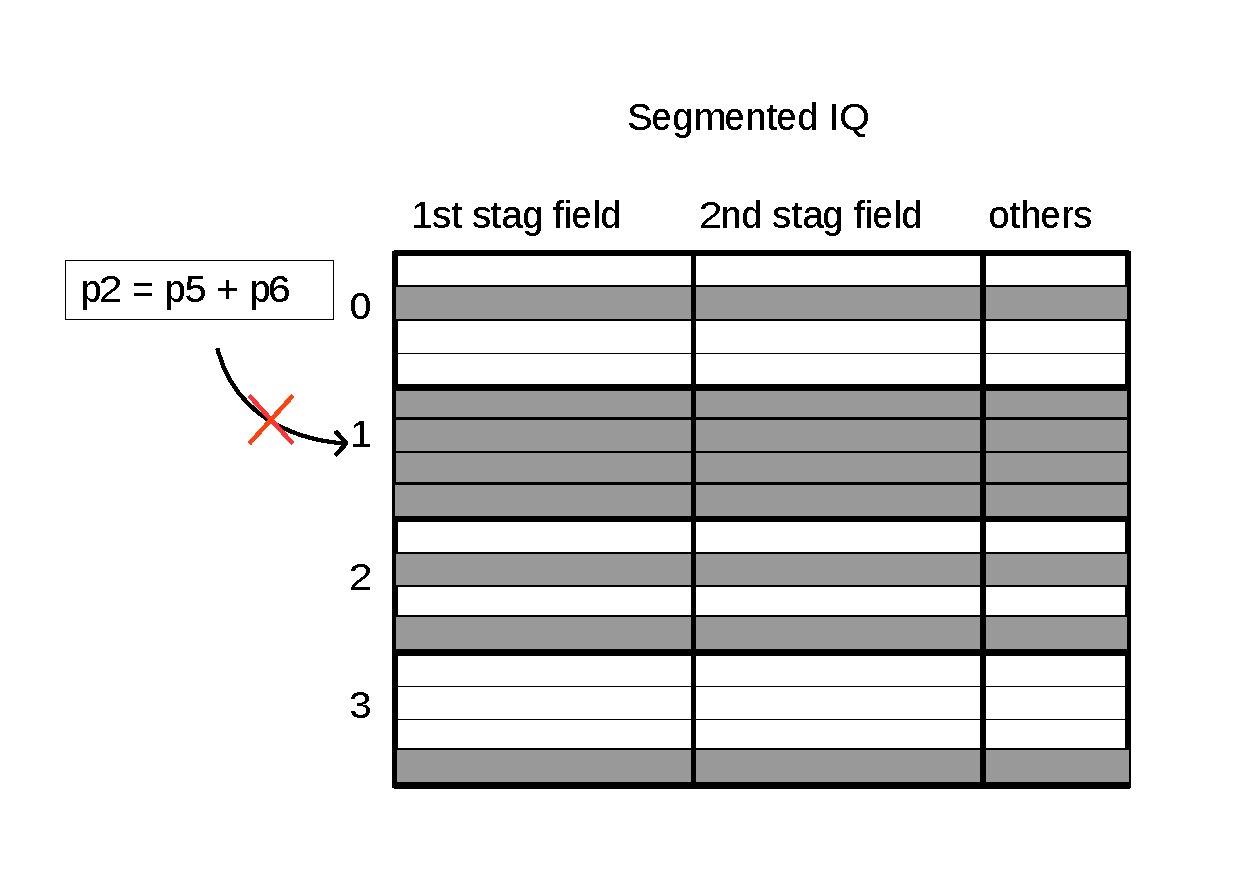
\includegraphics[keepaspectratio, scale=.8]{stall_segmentedIQ.pdf}
  \caption{容量効率が低下する例}
  \label{fig:stall_segmentedIQ}
\end{figure}

%5 提案手法による容量効率の低下
\section{容量効率の低下}
\label{sec:occupency_reduction}
提案手法には発行キューの容量効率が低下するという問題点がある.この問題点は,発行キューの容量効率が重要なプログラムにおいて,性能低下を引き起こす.本節では,容量効率が低下する原因について説明した後,容量効率の低下により性能低下を引き起こすプログラムの特徴に関して説明する.

\subsection{提案手法による容量効率低下の原因}
発行キューの容量効率の低下に関して,\fig{stall_segmentedIQ}を用いて説明する.図において,灰色のエントリは命令を保持していることを示している.

図の状態の発行キューに,新たに命令 $p2 = p5 + p6$ をディスパッチする場合を考える.この命令のソース・オペランドは両方レディでないとする.この場合,第 1 ソース・タグの下位ビットから第 1 セグメントにディスパッチされることが決定する.しかし,第 1 セグメントに空きエントリはないため,空きが出るまでディスパッチをストールさせ,待ち合わせを行う必要がある.

このように,命令がディスパッチされるセグメントに空きがない場合,他のセグメントに空きがあってもディスパッチをストールする必要があり,その結果,提案手法ではセグメント化されていない発行キューと比較して容量効率が低下する.

\subsection{容量効率の低下による性能低下}
プログラムには,性能が発行キューの容量に敏感なものとそうでないものとがある~\cite{Ando2019, Kora2013, Sembrant2015}.次の 2 つの特徴のうちいずれかに当てはまるプログラムでは,性能が発行キューの容量に敏感なため,与えられた発行キューの容量においては,その利用効率が重要である.このため,提案手法による容量効率の低下によって性能が低下する.
\begin{itemize}
  \item \textbf{命令レベル並列性(ILP:Instruction Level Parallelism)}が高いプログラム
  \item \textbf{メモリ・レベル並列性(MLP:Memory Level Parallelism)}が高いプログラム 
\end{itemize}

ILP が高いプログラムでは,できるだけ発行キューに命令を多く供給し,より多くの命令を並列に発行できるようにすることで高い性能が得られる.発行キューの容量効率が低下すると,並列に発行できる命令数が減少するため,性能が低下する.

MLP が高いプログラムでは,できるだけ多くのキャッシュ・ミスを並列に実行することにより,メモリ・アクセスのレイテンシが実行時間に与える影響を縮小できる.発行キューの容量効率が低下すると,並列に処理できるメモリ・アクセスが減少するため,性能が低下する.

これらのことから,ILP もしくは MLP が高い場合には,提案手法による容量効率の低下を最小限に抑える工夫が必要となる.

%5 容量効率の低下への対策:SWITCH 方式
\section{容量効率低下への対策:SWITCH 方式}
\label{sec:switch}
発行キューの容量効率低下による性能低下を抑制する方式として,\textbf{SWITCH} と呼ぶ方式を提案する.SWITCH 方式では,次のようにして性能低下を抑制する.
\begin{itemize}
  \item セグメント選択回路の選択アルゴリズムとして,容量効率は低下するが,タグ比較回数を多く削減できるような選択を行う \textbf{AGGRESSIVE モード} と,タグ比較回数の削減率は低下するが,容量効率が大きく低下しないような選択を行う \textbf{CONSERVATIVE モード} の 2 つを用意する.
  \item 実行プログラムの ILP 及び MLP を一定のインターバルで監視し,ILP もしくは MLP が高いと判断されたなら次のインターバルでは CONSERVATIVE モードでディスパッチし,そうでないなら AGGRESSIVE モードでディスパッチを行う.
\end{itemize}

本節では,まず 2 つのセグメント選択のアルゴリズムに関して説明を行う.その後,ILP 及び MLP の評価方法と,切り替えアルゴリズムに関して説明する.

\subsection{2 つのセグメント選択アルゴリズム}
SWITCH 方式では,タグ比較回数の削減重視の AGGRESSIVE モードと,容量効率重視の CONSERVATIVE モードの 2 つを適切に切り替えて使用する.各モードには,タグ比較回数の削減と容量効率に関して,\tab{switch_trade_off}に示すトレード・オフの関係がある.それぞれのセグメントの選択方法に関して説明する.

なお, SWITCH 方式はサブ・セグメント方式と併用が可能であるが,説明を簡単にするため,サブ・セグメントを使用しない場合に関して説明する.サブ・セグメントと SWITCH 方式を併用するような拡張は容易に行うことができる.

\begin{table}[tb]
  \caption{2 つのセグメント選択モードのトレード・オフ}
  \footnotesize
  \center
   \begin{tabular}{l|c|c} \hline \hline
   モード & タグ比較回数の削減 & 容量効率 \\ \hline
   AGGRESSIVE & ○ & × \\
   CONSERVATIVE & × & ○ \\ \hline
  \end{tabular}
  \label{tab:switch_trade_off}
\end{table}

\subsubsection{AGGRESSIVE モード}
AGGRESSIVE モードは,\ref{sec:swap}節で示した選択アルゴリズムを使用してディスパッチするエントリを決定する.このモードでは,選択されたセグメントに空きがない場合,他のセグメントに空きがあってもディスパッチは行わないため,容量効率が低下する.しかし,セグメント化の利益を最大限利用し,タグ比較回数を大幅に削減できる.

\subsubsection{CONSERVATIVE モード}
AGGRESSIVE モードでは,命令のソース・オペランドが両方レディであり,セグメント・インディペンデントとしてディスパッチできる場合以外では,ソース・タグによって選択されるセグメントに空きがない場合にディスパッチをストールさせる.これに対し,CONSERVATIVE モードでは,以下で説明する工夫を行うことによって,このディスパッチのストールを回避し,容量効率の低下を抑制する.
\begin{itemize}
  \item \textbf{両ソース・オペランドともレディでない場合}:\\AGGRESSIVE モードでは第 1 ソース・タグの下位ビットによってセグメントを選択する.選択されたセグメントに空きがない場合,ディスパッチを行わない.これに対して CONSERVATIVE モードでは,第 1 ソース・タグによって選択されたセグメントに空きがない場合には,\textbf{スワップ}~\footnote{\ref{sec:swap}節では,スワップの定義を「第 1 ソース・オペランドのみレディの場合に,第 1 ソース・タグと第 2 ソース・タグを書き込むフィールドを交換する」としていたが,本節以降ではこの定義を拡大し,単に「第 1 ソース・タグと第 2 ソース・タグを書き込むフィールドを交換する」という意味で用いる.}\textbf{して}ディスパッチを試みる.スワップするため,第 2 ソース・タグにより選択されるセグメントに空きがあればディスパッチが可能となる.
  \item \textbf{第 1 ソース・オペランドのみレディである場合}:\\AGGRESSIVE モードでは,スワップを行い,第 2 ソース・タグでセグメントを選択する.選択されたセグメントに空きがない場合,ディスパッチを行わない.これに対して CONSERVATIVE モードでは,第 2 ソース・タグによって選択されたセグメントに空きがない場合には,\textbf{スワップをやめて}ディスパッチする.スワップをやめるため,第 1 ソース・タグによってセグメントが選択されるが,第 1 ソース・オペランドは既にレディであるため,どのセグメントにディスパッチしても良い.従って,セグメント・インディペンデントとしてディスパッチが可能となる.
  \item \textbf{第 2 ソース・オペランドのみレディである場合}:\\AGGRESSIVE モードでは第 1 ソース・タグでセグメントを選択する.選択されたセグメントに空きがない場合,ディスパッチを行わない.これに対して CONSERVATIVE モードでは,第 1 ソース・タグによって選択されたセグメントに空きがない場合には,\textbf{スワップして}ディスパッチする.スワップするため,第 2 ソース・タグによってセグメントが選択されるが,第 2 ソース・オペランドは既にレディであるため,どのセグメントにディスパッチしても良い.従って,セグメント・インディペンデントとしてディスパッチが可能となる.
\end{itemize}
上述の工夫によって,CONSERVATIVE モードでは,どちらかのソース・オペランドがレディである場合は,必ずディスパッチが可能となる.また,両ソース・オペランドともレディでない場合でも,第 1 ソース・タグにより選択されるセグメントと第 2 ソース・タグにより選択されるセグメントのうち,いずれかのセグメントに空きがあればディスパッチが可能となる.従って,ストールする確率は大きく減少する.

以下に,CONSERVATIVE モードにおけるセグメントの選択アルゴリズムをまとめる.
\begin{itemize}
  \item \textbf{両ソース・オペランドともレディでない場合}:第 1 ソース・タグでセグメントを選択する.選択したセグメントに空きがない場合,スワップして第 2 ソース・タグをもとにセグメントを決定する.なおも空きがない場合はストールする.
  \item \textbf{第 1 ソース・オペランドのみレディである場合}:スワップを行い,第 2 ソース・タグでセグメントを選択する.選択したセグメントに空きがない場合は,スワップをやめて,セグメント・インディペンデントとしてラウンドロビンでセグメントを選択する.
  \item \textbf{第 2 ソース・オペランドのみレディである場合}:第 1 ソース・タグでセグメントを選択する.選択したセグメントに空きがない場合はスワップを行い,セグメント・インディペンデントとしてラウンドロビンでセグメントを選択する.
  \item \textbf{両ソース・オペランドがレディである場合}:セグメント・インディペンデントとしてラウンドロビンでセグメントを選択する.
\end{itemize}

\subsubsection{CONSERVATIVE モードにおけるタグ比較回数の削減}
CONSERVATIVE モードでは,AGGRESSIVE モードと比較してタグ比較回数の削減率が 低下する可能性がある.この理由について説明する.例として,第 2 ソース・オペランドのみレディである命令をディスパッチする場合について説明する.

CONSERVATIVE モードでは,まず第 1 ソース・タグでセグメントを選択する.選択されたセグメントに空きがあれば,そのセグメントにディスパッチする.この場合,レディでない第 1 ソース・タグが,セグメント化によってタグ比較回数が削減される第 1 ソース・タグのフィールドに書き込まれるため,AGGRESSIVE モードと同様にタグ比較回数が削減される.

第 1 ソース・タグによって選択されたセグメントに空きがなければ,CONSERVATIVE モードではスワップしてセグメント・インディペンデントとしてディスパッチする.この場合,タグ比較回数の削減は行うことができない.これは,既にレディである第 2 ソース・オペランドのタグが,セグメント化によってタグ比較回数を削減できる第 1 ソース・タグのフィールドに書き込まれ,一方で,まだレディでなくタグ比較が行われる第 2 ソース・オペランドのタグが,セグメント化によってタグ比較回数が削減されない第 2 ソース・タグのフィールドに書き込まれるためである.

AGGRESSIVE モードでは,第 1 ソース・タグによって選択されたセグメントに空きがなければ,ストールして空きが出るまで待ち合わせる.このストールにより,容量効率は低下するが,空きが出たあとディスパッチするため,タグ比較回数は削減される.これに対して CONSERVATIVE モードでは,タグ比較回数の削減は行えなくなるが,スワップしてディスパッチすることによってストールを回避し,容量効率の低下を防ぐ.

従って,CONSERVATIVE モードは,タグ比較回数の削減をある程度犠牲にして,発行キューの容量効率の低下を抑制するアルゴリズムであるといえる.

\subsection{モードの切り替え}
SWITCH 方式では, AGGRESSIVE と CONSERVATIVE の 2 つのモードを,実行プログラムの ILP や MLP の量に応じて切り替えて使用する.ここで重要となるのは ILP や MLP の量の評価方法である.本研究では, ILP の評価方法として Issue Stall Rate(ISR) という評価値を使用する.また, MLP の評価方法としては,最終レベル・キャッシュ(LLC: last-level cache)の MPKI(misses per kilo instructions)を使用する.それぞれに関して詳しく説明した後,切り替えアルゴリズムを説明する.

\subsubsection{Issue Stall Rate(ISR)}
ISR は,「インターバルの全サイクルのうち 1 命令も発行されないサイクルの割合」を表す指標である.ILP が高い場合,多くのサイクルで命令が発行されるため,ISR は低い値を示す.一方, ILP が低い場合には,命令が発行されないサイクルが一定の割合で発生するため,ISR は高くなる.

あらかじめISR にしきい値を設け,インターバルでの ISR がしきい値を下回った場合に ILP が高いと判断し,そうでなければ低いと判断する.

\subsubsection{LLC MPKI}
LLC MPKI は LLC のキャッシュ・ミスの発生頻度を表す指標である.LLC MPKI があらかじめ定めたしきい値を上回った場合に MLP が高いと判断し,そうでなければ低いと判断する.

\begin{figure}[htb]
  \centering
  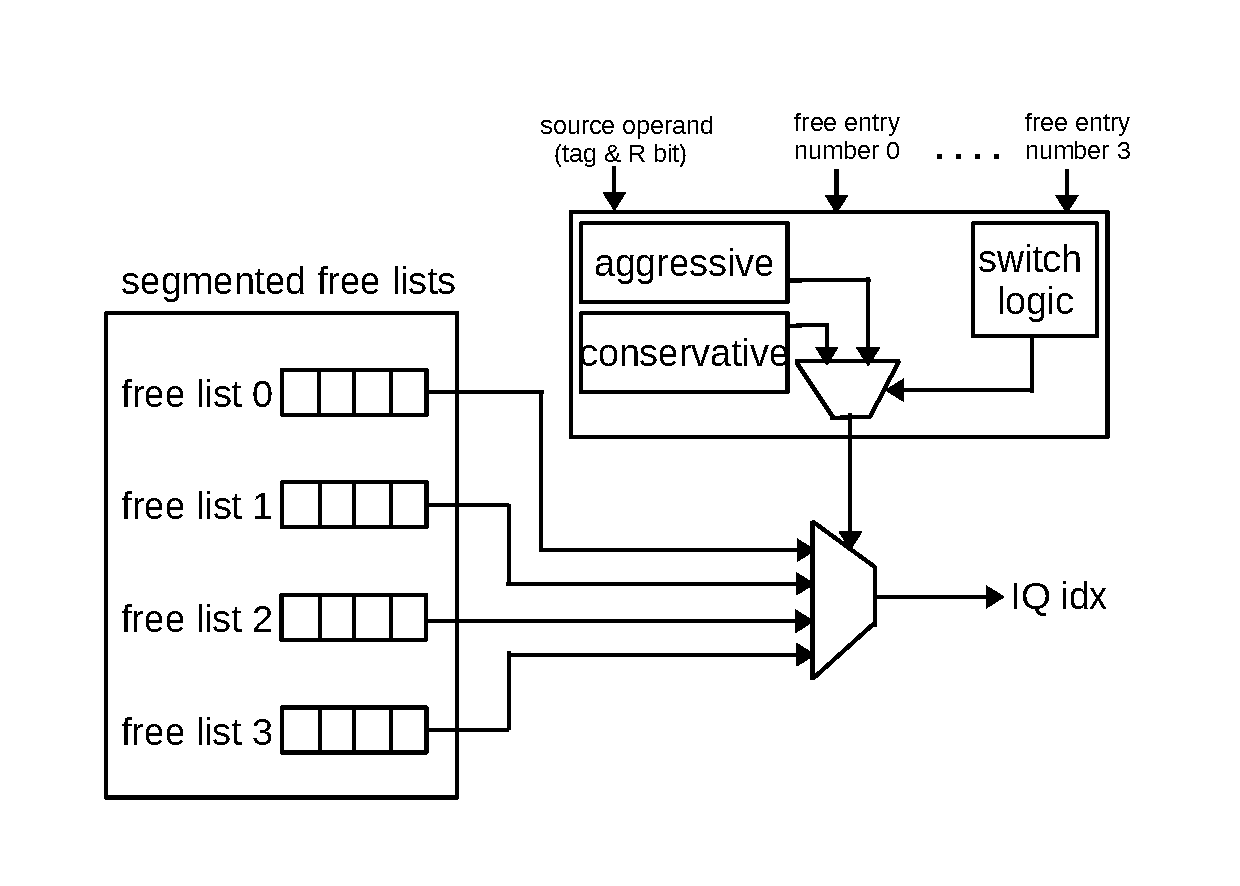
\includegraphics[keepaspectratio, scale=.8]{switch.pdf}
  \caption{SWITCH 方式におけるディスパッチエントリの決定回路}
  \label{fig:switch}
\end{figure}

\subsubsection{切り替えアルゴリズム}
切り替えアルゴリズムは以下に示すとおりである.一定のインターバルにおいて,ISR と LLC MPKI を測定し,ILP および MLP の高低を判断する.ILP または MLP のいずれかが高いと判定された場合,次のインターバルを CONSERVATIVE モードで実行する.ILP と MLP がどちらも低いと判定された場合,次のインターバルを AGGRESSIVE モードで実行する.

SWITCH 方式におけるディスパッチするエントリの決定回路を\fig{switch}に示す.AGGRESSIVE と CONSERVATIVE の 2 つの選択アルゴリズムのうち,どちらを利用するかを SWITCH 回路が選択し,その結果に応じてセグメントが選択される.

\begin{figure*}[htb]
  \centering
  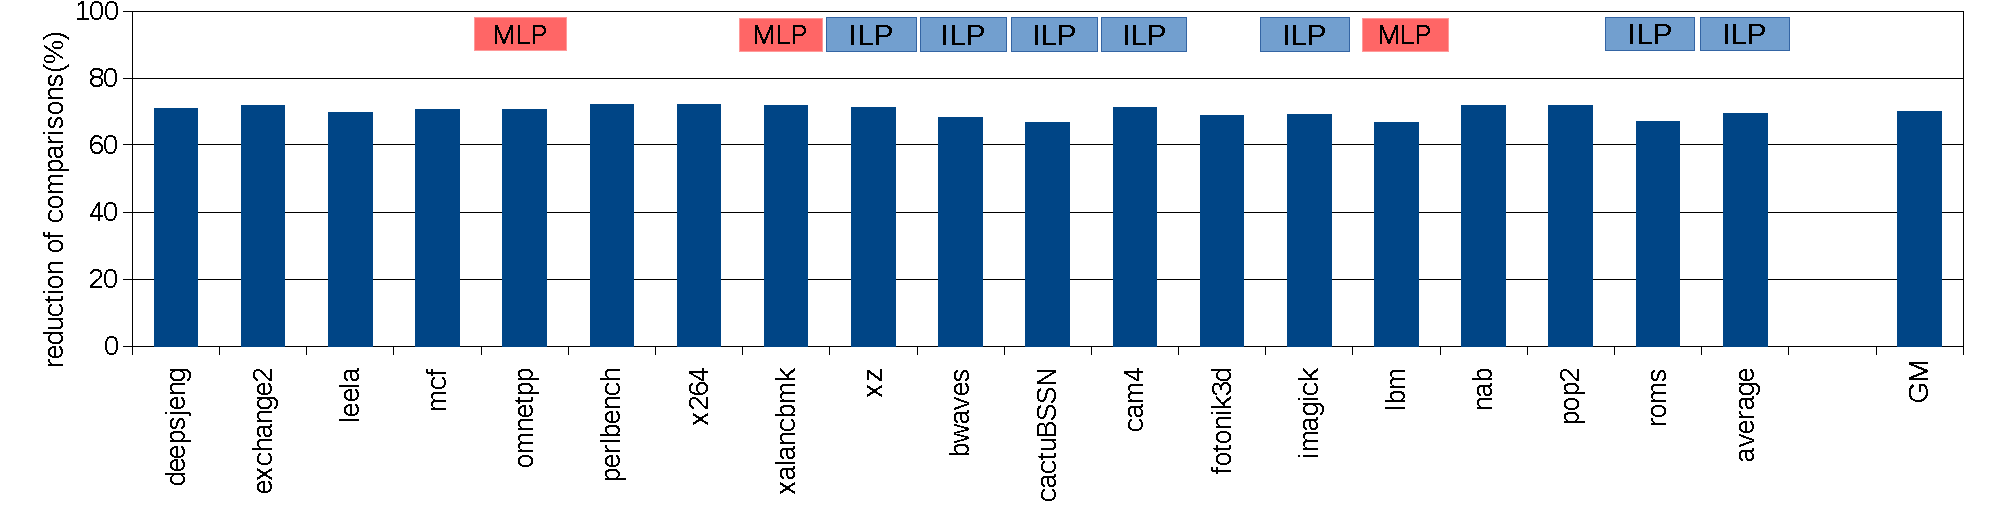
\includegraphics[width=0.99\hsize]{comp.pdf}
  \caption{提案手法によるタグ比較削減}
  \label{fig:comp}

  \vspace{0.5cm}

  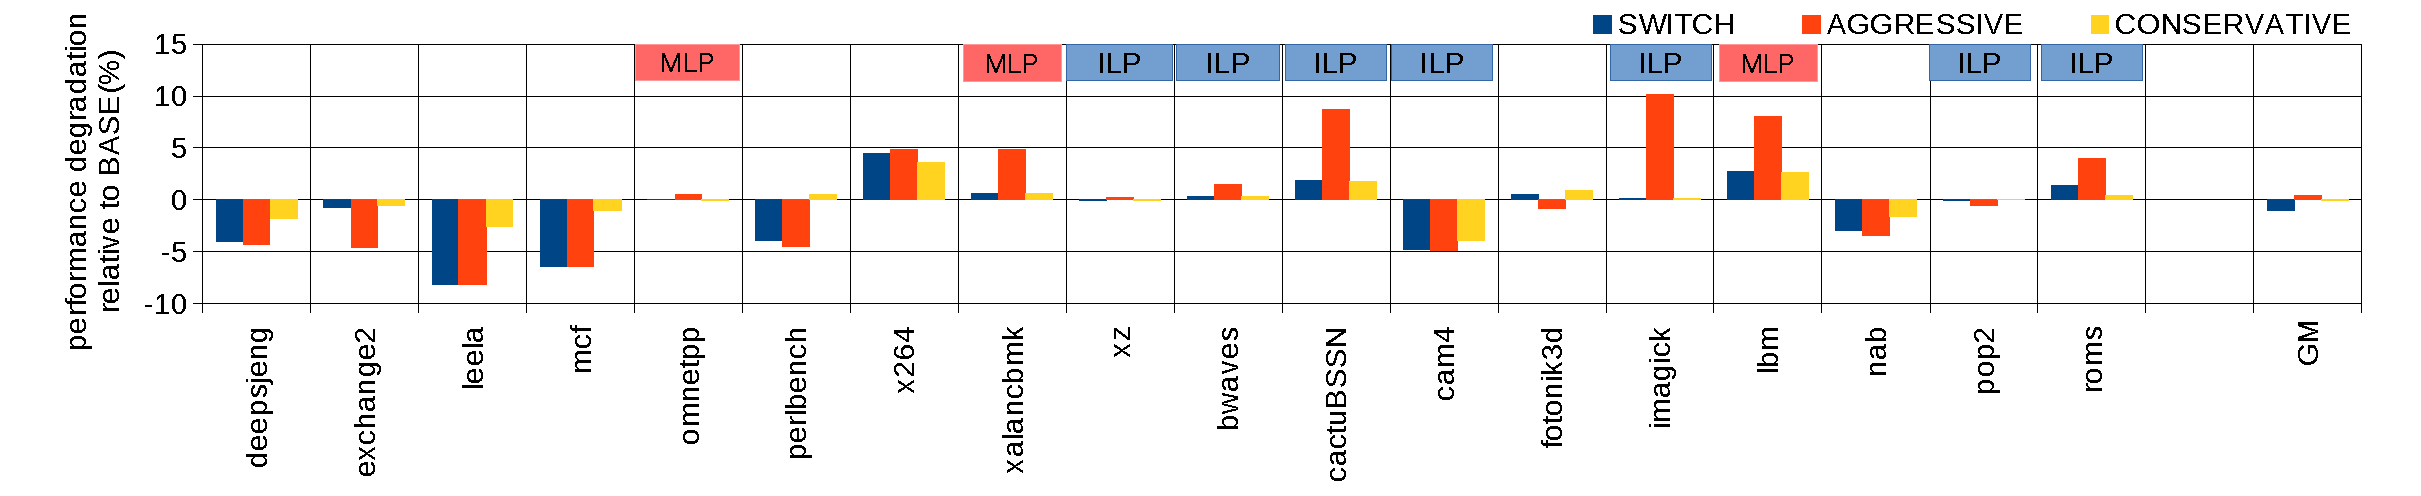
\includegraphics[width=0.99\hsize]{IPC.pdf}
  \caption{提案手法による性能低下}
  \label{fig:IPC}

  \vspace{0.5cm}

  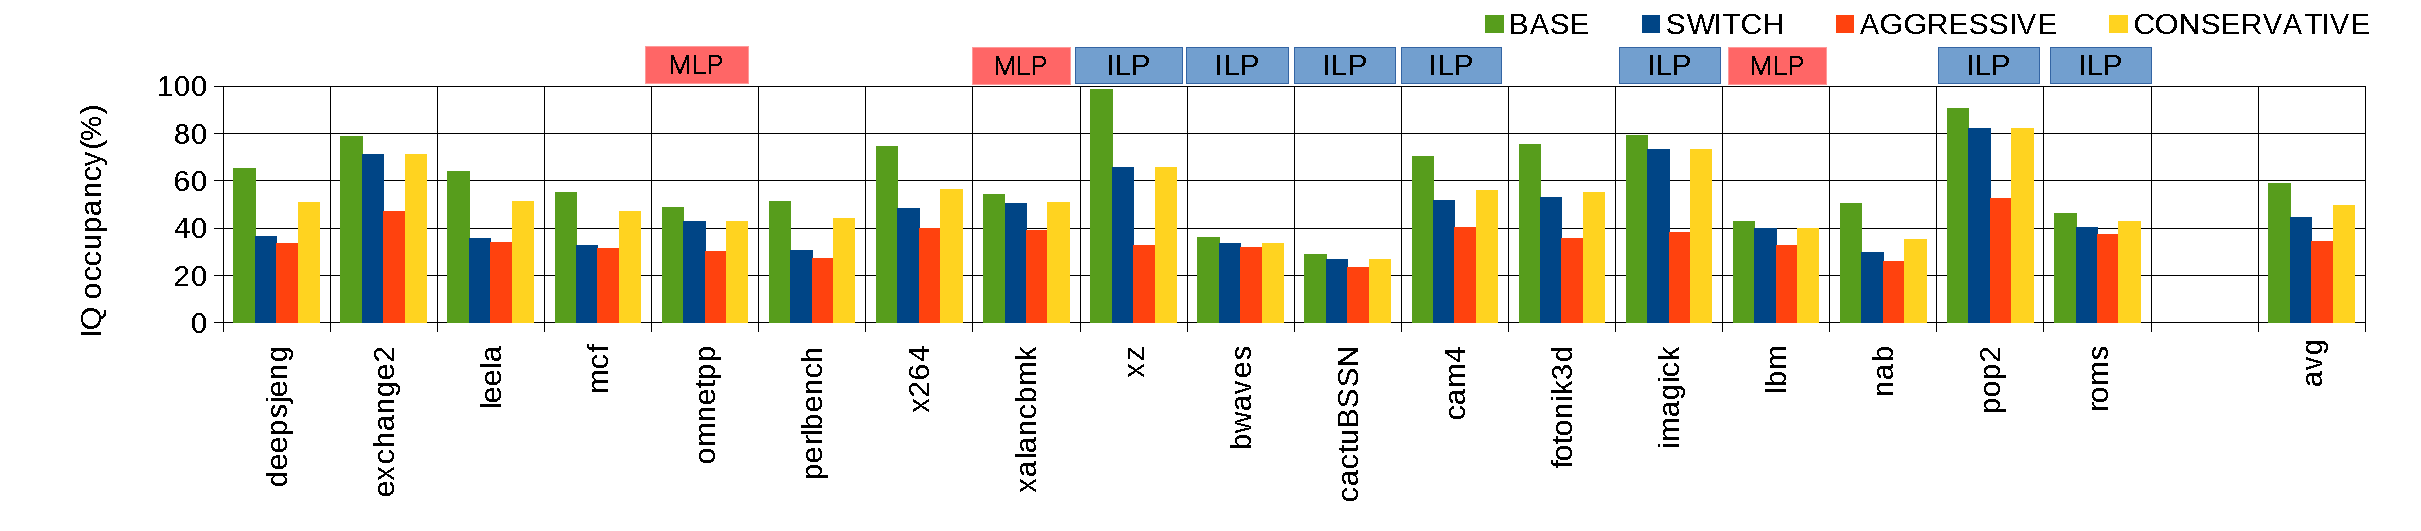
\includegraphics[width=0.99\hsize]{IQ_occupency.pdf}
  \caption{提案手法による容量効率の変化}
  \label{fig:IQ_occupency}
\end{figure*}

%6 評価
\section{評価}
\label{sec:eval}
\subsection{評価環境}
評価環境について説明する.性能やタグ比較回数を評価するために,SimpleScalar v.3.0a をベースに作成したシュミレータを使用した.評価で仮定したプロセッサ構成を\tab{base_config}に示す.

提案手法の各種パラメータを,\tab{segmentedIQ_config}に示す.5\% 程度の性能低下と引き換えにできるだけ多くのタグ比較回数削減を達成できるよう,実験によって求めた最適なパラメータである.セグメント数の違いによるタグ比較回数の削減及び性能低下に関しては,\ref{sec:ipc_comp}節で評価を行う.

測定ベンチマークには,SPEC CPU 2017 ベンチマークのうち,int 系 9 本と fp 系 9 本の計 18 本を使用した.ベンチマークの測定区間は,プログラムの先頭から 16B 命令をスキップした後の 100M 命令である.

\begin{table}[htb]
  \caption{プロセッサの基本構成}
  \footnotesize
  \center
    \begin{tabular}{l|l} \hline \hline
     Pipeline width & 8 instructions wide for each of \\
     & fetch, decode, issue, and commit \\
     Reorder buffer & 300 entries \\
     IQ & 128 entries \\
     Load/Store queue & 128 entries \\
     Physical registers & 300(int) + 300(fp) \\
     Branch prediction & 16KB Perceptron predictor~\cite{Jimenez2001} \\
     & 2K-set 4-way BTB \\
     & 10-cycle misprediction penalty \\
     Function unit & 4 iALU, 2 iMULT, \\
     &  3 FPU, 2 LSU \\
     L1 D-cache & 32KB, 8-way, 64B line \\
      & 2-cycle hit latency \\
     L1 I-cache & 32KB, 8-way, 64B line \\
      &  2-cycle hit latency \\
     L2 cache & 2MB, 16-way, 64B line \\
      & 12-cycle hit latency \\  
     Main memory & 300-cycle latency \\
     & 8B/cycle bandwidth \\ 
     Prefetch & stream-based,32-stream tracked,  \\ 
     & 16-line distance, 2-line degree, \\
     & prefetch to L2 cache \\ \hline
  \end{tabular}
  \label{tab:base_config}
\end{table}

\begin{table}[htb]
  \caption{提案手法のパラメータ構成}
  \footnotesize
  \center
    \begin{tabular}{l|l} \hline \hline
    メイン・セグメント数 & 16 \\
    サブ・セグメント数 & 2 \\
    切り替えインターバル & 10K instructions \\
    ISR しきい値 & 15\% \\
    LLC MPKI しきい値 & 2.0 \\ \hline 
  \end{tabular}
  \label{tab:segmentedIQ_config}
\end{table}

\subsection{評価モデル}
評価した4種類のプロセッサ・モデルを示す.
\begin{itemize}
  \item \textbf{BASE}: 提案手法を用いない基準のモデル
  \item \textbf{SWITCH}: 提案手法において SWITCH 方式によるモード切り替えを行うモデル
  \item \textbf{AGGRESSIVE}: 提案手法において常に AGGRESSIVE モードで実行するモデル
  \item \textbf{CONSERVATIVE}: 提案手法において常に CONSERVATIVE モードで実行するモデル
\end{itemize}

\subsection{評価結果}
\subsubsection{タグ比較回数の削減}
\fig{comp}に,提案手法の BASE モデルに対するタグ比較回数の割合をベンチマークごとに示す.なお,各棒グラフの上の ILP 及び MLP の表記は,それぞれ,そのベンチマークが ILP または MLP が高いベンチマークであることを示している.ここで,ILP が高いとは BASE モデルでの IPC が 3.5 以上であることを表し,MLP が高いとは BASE モデルでの LLC MPKI が 2.0 以上であることを表す. 

AGGRESSIVE と CONSERVATIVE のタグ比較回数削減に関しては,同図より,いずれのベンチマークにおいても,AGGRESSIVE のほうがタグ比較回数が少ないことがわかる.その差は 平均で 10\% 程度となっており,AGGRESSIVE モードのタグ比較回数を積極的に削減できるという性質が確認できる.

同図より SWITCH 方式では,平均で BASE モデルの 15\% 程度のタグ比較回数となっており,85\% の削減を達成している.

SWITCH 方式では,ILP や MLP の高いベンチマークにおいてはCONSERVATIVE と同程度のタグ比較回数であるのに対して,そうでないベンチマークにおいては AGGRESSIVE と同程度のタグ比較回数となっていることがわかる.したがって,発行キューの容量効率が重要でないベンチマークにおいては,AGGRESSIVE モードを選択して積極的にタグ比較回数の削減が行えていることがわかる.

\subsubsection{性能低下}
\fig{IPC}に,BASE に対する提案手法による性能低下をベンチマークごとに示す.同図より,SWITCH 方式による性能低下は最大で 5\% 程度であり,多くのベンチマークでは 0\% に近く性能はほとんど低下しないということが確認できる.

SWITCH 方式の有効性に関して述べる.同図より,ILP や MLP が高い cactusBSSN や imagick,lbm などのベンチマークにおいて,AGGRESSIVE では大きく性能低下しているのに対して,CONSERVATIVE では性能低下が抑制されていることが分かる.そして SWITCH では,CONSERVATIVE と同程度の性能低下にとどまっている.従って,容量効率が性能にとって重要なプログラムにおいて,SWITCH 方式によって性能低下が抑制できていることが分かる.

\fig{IQ_occupency}に各モデルでの発行キューの占有率を示す.占有率とは,発行キューの全エントリのうち使用された割合であり,この値が BASE のそれに近いほど容量効率が低下していないことを示す.

同図より,AGGRESSIVE では BASE に対して占有率が大きく低下しているのに対して, CONSERVATIVE では占有率の低下がある程度抑制できていることが分かる.そして,ILP や MLP が高いベンチマークでは SWITCH 方式での占有率が CONSERVATIVE と同程度となっていることが分かる.このことからも,SWITCH 方式では,容量効率の性能に対する重要性に応じて適切にモードを選択し,容量効率の低下による性能低下を抑制できており, SWITCH 方式が有効であるとわかる.

\fig{IPC}より,いくつかのベンチマークでは性能が向上していることが分かる.この理由に関して説明する.一般にランダム・キュー方式の発行キューには,命令がプログラム順に並んでいないため,最も優先して発行すべき命令の発行が遅れる可能性があるという欠点が存在する.ランダム・キューでは,命令の並びが年齢についてランダムになる一方,選択論理は,下のエントリほど優先して発行命令を選択するため,レディ命令が発行幅以上に存在する発行コンフリクトが生じた場合,誤った優先度で命令を選択することが生じる.
提案手法では発行キューの容量効率が低下するため,発行キュー内の命令数が少なくなり,結果的に発行コンフリクトが生じる確率が低下し,問題が生じにくくなり,性能が向上する.

\begin{figure}[htb]
  \centering
  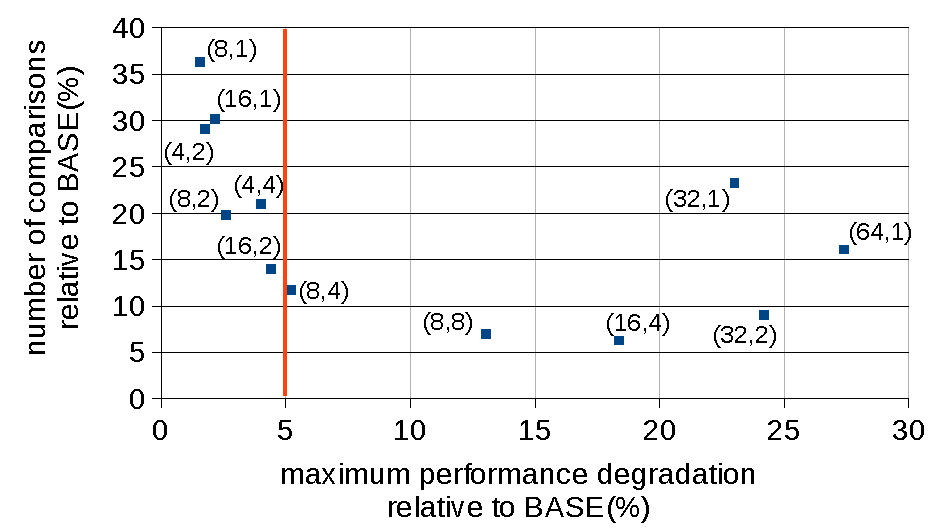
\includegraphics[keepaspectratio, scale=.55]{ipc_comp.pdf}
  \caption{セグメント数の違いによるタグ比較回数の削減と性能低下}
  \label{fig:ipc_comp}
\end{figure}

\subsubsection{セグメント数に関する評価}
\label{sec:ipc_comp}
\fig{ipc_comp}に,メイン・セグメント数とサブ・セグメント数を変化させた場合の,SWITCH 方式での性能低下とタグ比較回数の散布図を示す.図中の各点にはメイン・セグメント数とサブ・セグメント数を(M-seg,S-seg)という形式で付与している.横軸は最も性能低下が大きかったベンチマークにおける性能低下を示し,縦軸は全ベンチマークでの平均のタグ比較回数を示す.

同図より,セグメントの総数が増えると,タグ比較回数はより削減されるが,同時に性能低下も大きくなることがわかる.また,セグメントの総数が同じ場合((16, 1)と(8, 2)など),サブ・セグメントを利用するほうが,よりタグ比較回数を削減できていることが分かる.このことから,サブ・セグメント方式は有効であるといえる.

本論文では,性能低下は全てのベンチマークで 5\% 以下に抑えるという基準を設定している.従って,\fig{ipc_comp}において性能低下が 5\% より小さいセグメント数の組み合わせのうち,最もタグ比較回数が削減される(16,2)を最適であると判断した.

%7 まとめ
\section{まとめ}
\label{sec:summary}
LSIの微細化の進展に伴って,経年劣化が加速し摩耗故障が増加する問題が深刻になっている.この故障は,デバイスの温度に関して指数関数的に加速するため,チップ内のホット・スポットの解消が求められている.

発行キューはこのホット・スポットの 1 つとして知られている.この主な原因はウェイクアップ時の多数のタグ比較である.本論文では,ウェイクアップ時のタグ比較回数を削減するために,発行キューをセグメント化,および,それに関わるいくつかの手法を提案した.

提案手法には発行キューの容量効率が低下するという問題点が存在する.この問題点に対して,本論文ではさらに,異なる 2 つのディスパッチ・アルゴリズムを,性能についての容量効率の重要性に応じて切り替えて使用することにより,容量効率の低下による性能低下を抑制する手法を提案した.提案手法を SPEC CPU 2017 を使って評価したところ,性能低下を最大でも 5\% 以下(平均 -1\%)に抑えつつ,タグ比較回数を 85\% 削減できることを確認した.

\begin{acknowledgment}
本研究は,JSPS科研費20K11732の助成を受けたものです.
\end{acknowledgment}

%参考文献
\bibliographystyle{ipsjunsrt}
\bibliography{ref}

\end{document}
